\chapter{C++编程基础}

由于这只是一个有关机器人足球的技术文档,不在这里赘述过多C++知识,
仅在此提供一个由c语言基础过度到C++的简易教程。更多的知识请参照
C++ primer plus。\footnote{<<C++ primer plus (第6版)>> }
\section{c++对c的扩充}
\subsection{文件名称}
在C语言中,源文件的拓展名为”.c”,头文件的拓展名为”.h”,在C++语言中源文件的拓展名由“.c”变更为了”.cpp”,而头文件依然可以使用C语言中的拓展名”.h”

在使用include对文件进行包含时,C语言需要加上文件”.h”拓展名而C++则可以仅使用文件名。

C语言文件包含

\begin{Code}
#include<iostream.h>
\end{Code}

C++文件包含
\begin{Code}
#include<iostream>
\end{Code}

由于C++为C语言发展而来,C++保留了一部分C的规定,使得C++可以很好的兼容C语言,所以在C++中以下文件的包含方式也是可以的。

C++文件包含
\begin{Code}
#include<iosteam.h>
\end{Code}
\subsection{命名空间}
命名空间为面向对象程序设计的重要概念之一,他可以通过将用户定义的函数或类放置在一个命名空间中的方法来防止用户定义的函数或类与他人的定义发生重名。

命名空间的定义:

\begin{Code}
namespace 名称
{
	内容
}
\end{Code}

命名空间的访问:

\begin{Code}
名称::内容
\end{Code}

命名空间的使用:

\begin{Code}
using namespace 名称;
\end{Code}

\subsection{标准输入输出}
C++在进行输入及输出时除了可以使用C语言中的prinyf与scanf函数外,还可以使用C++中提供的cin和cout流对象。

\subsubsection{使用cout进行输出}
在使用cout进行输出时需要在被输出项前加<<符号,需要注意的是每一个输出项使用一个<<符号而不可以多个输出项共用一个。并且如果在输出时没有指定输出的数据类型的话,系统会以输出项被定义的类型进行输出。


\begin{Code}
int a = 1;
float b = 3.5;
char c = ‘x’

正确输出方式 cout << a << b << c;
错误输出方式 cout << a,b,c;
输出结果:13.5x
\end{Code}

\subsubsection{使用cin进行输入}



\subsection{动态内存分配与释放}
C/C++定义了4个内存区间:
代码区,全局变量与静态变量区,局部变量区即栈区,动态存储区,即堆(heap)区或自由存储区(free store)。

\subsubsection{堆的概念}
通常定义变量(或对象),编译器在编译时都可以根据该变量(或对象)的类型知道所需内存空间的大小,从而系统在适当的时候为他们分配确定的存储空间。这种内存分配称为静态存储分配;
有些操作对象只在程序运行时才能确定,这样编译时就无法为他们预定存储空间,只能在程序运行时,系统根据运行时的要求进行内存分配,这种方法称为动态存储分配。所有动态存储分配都在堆区中进行。

当程序运行到需要一个动态分配的变量或对象时,必须向系统申请取得堆中的一块所需大小的存贮空间,用于存贮该变量或对象。当不再使用该变量或对象时,也就是它的生命结束时,要显式释放它所占用的存贮空间,这样系统就能对该堆空间进行再次分配,做到重复使用有限的资源。
\subsubsection{堆内存的分配与释放}
\textbf{堆空间申请、释放的方法:}

在C++中,申请和释放堆中分配的存贮空间,分别使用new和delete的两个运算符来完成:

\begin{Code}
指针变量名=new 类型名(初始化式);
delete 指针名;
\end{Code}
例如:
\begin{Code}
int *pi=new int(0);
\end{Code}

它与下列代码序列大体等价:
\begin{Code}
int ival=0, *pi=&ival;
\end{Code}
区别:pi所指向的变量是由库操作符new()分配的,位于程序的堆区中,并且该对象未命名。  

\textbf{堆空间申请、释放说明:}

\begin{enumerate}
	\item new运算符返回的是一个指向所分配类型变量(对象)的指针。对所创建的变量或对象,都是通过该指针来间接操作的,而且动态创建的对象本身没有名字。
	\item 一般定义变量和对象时要用标识符命名,称命名对象,而动态的称无名对象(请注意与栈区中的临时对象的区别,两者完全不同:生命期不同,操作方法不同,临时变量对程序员是透明的)。
	\item 堆区是不会在分配时做自动初始化的(包括清零),所以必须用初始化式(initializer)来显式初始化。new表达式的操作序列如下:从堆区分配对象,然后用括号中的值初始化该对象。
\end{enumerate}

\subsubsection{堆空间申请、释放演示}

\begin{enumerate}
	\item 用初始化式(initializer)来显式初始化
	
	int *pi=new int(0);
	\item 当pi生命周期结束时,必须释放pi所指向的目标:
	
	delete pi;
	
	注意这时释放了pi所指的目标的内存空间,也就是撤销了该目标,称动态内存释放(dynamic memory deallocation),但指针pi本身并没有撤销,它自己仍然存在,该指针所占内存空间并未释放。
\end{enumerate}
下面是关于new操作的说明
\begin{enumerate}
	\item new运算符返回的是一个指向所分配类型变量(对象)的指针。对所创建的变量或对象,都是通过该指针来间接操作的,而动态创建的对象本身没有名字。
	
	\item 一般定义变量和对象时要用标识符命名,称命名对象,而动态的称无名对象(请注意与栈区中的临时对象的区别,两者完全不同:生命期不同,操作方法不同,临时变量对程序员是透明的)。
	\item 堆区是不会在分配时做自动初始化的(包括清零),所以必须用初始化式(initializer)来显式初始化。new表达式的操作序列如下:从堆区分配对象,然后用括号中的值初始化该对象。
	
	在软件开发过程中,常常需要动态地分配和撤销内存空间,例如对动态链表中结点的插入与删除。在C语言中是利用库函数malloc和free来分配和撤销内存空间的。C++提供了较简便而功能较强的运算符new和delete来取代malloc和free函数。
\end{enumerate}


注意: new和delete是运算符,不是函数,因此执行效率高。

虽然为了与C语言兼容,C++仍保留malloc和free函数,但建议用户不用malloc和free函数,而用new和delete运算符。new运算符的例子:
\begin{Code}
new int;  //开辟一个存放整数的存储空间,返回一个指向该存储空间的地址(即指针)
new int(100);  //开辟一个存放整数的空间,并指定该整数的初值为100,返回一个指向该存储空间的地址
new char[10];  //开辟一个存放字符数组(包括10个元素)的空间,返回首元素的地址
new int[5][4];  //开辟一个存放二维整型数组(大小为5*4)的空间,返回首元素的地址
float *p=new float (3.14159);  //开辟一个存放单精度数的空间,并指定该实数的初值为
			//3.14159,将返回的该空间的地址赋给指针变量p
\end{Code}
\textbf{new运算符}使用的一般格式为:

new 类型 [初值];

用new分配数组空间时不能指定初值。如果由于内存不足等原因而无法正常分配空间,则new会返回一个空指针NULL,用户可以根据该指针的值判断分配空间是否成功。

\textbf{delete运算符}使用的一般格式为:

delete [ ] 指针变量

例如要撤销上面用new开辟的存放单精度数的空间(上面第5个例子),应该用
delete p;

前面用“new char[10];”开辟的字符数组空间,如果把new返回的指针赋给了指针变量pt,则应该用以下形式的delete运算符撤销该空间:
\begin{Code}
delete [] pt;  //在指针变量前面加一对方括号,表示是对数组空间的操作
\end{Code}
\subsection{函数新特性}
\subsubsection{函数原型 }
在C++中要求为每一个函数建立一个原型,用以说明函数的名称、参数个数及类型和函数的返回值的类型。
其主要目的是让C++编译程序进行类型检查,即形参与实参的类型匹配检查,以及返回值是否与原型相符,以维护程序的正确性。所以应该养成将声明和定义分开编写的好习惯。
函数原型与函数定义要在函数的返回类型,函数名和函数参数类型及数量这三个方面保持一致。
在写函数原型时,可以省略形参的名字,因为参数的名字对于编译器没有意义,但如果取名恰当的话,这些名字可以起到提示参数用途的作用。
\subsubsection{函数内联}
一般情况下,我们对内联函数做如下的限制:
(1) 不能有递归
(2) 不能包含静态数据
(3) 不能包含循环
(4) 不能包含switch和goto语句
(5) 不能包含数组
若一个内联函数定义不满足以上限制,则编译系统把它当作普通函数对待。
函数缺省参数
如果在函数说明或函数定义中为形参指定一个缺省值,则称此函数为带缺省参数的函数。当函数调用发生后,在形参表中等号后的各“缺省值”将起实参的传递作用。
如果函数有多个缺省参数,则缺省参数必须是从右向左定义,并且在一个缺省参数的右边不能有未指定缺省值的参数。

void fun(int a,int b,int c,int d=5);          
fun(1,2,3)

void fun(int a=65,int b=3,int c,int d=3);     //错误

如果在函数原型的声明中设置了函数参数的缺省值,则不可再在函数定义的头部重复设置,否则编译时将出现错误信息。
\subsubsection{函数重载}
C++编译系统允许为两个或两个以上的函数取相同的函数名,但是形参的个数或者形参的类型不应相同,编译系统会根据实参和形参的类型及个数的最佳匹配,自动确定调用哪一个函数,这就是所谓的函数重载。
函数重载无需特别声明,只要所定义的函数与已经定义的同名函数形参形式不完全相同,C++编译器就认为是函数的重载。

不可以定义两个具有相同名称、相同参数类型和相同参数个数,只是函数返回值不同的函数。
int func(int x);
float func(int x);

如果某个函数参数有缺省值,必须保证其参数缺省后调用形式不与其它函数混淆。
int f(int a, float b);
void f(int a, float b, int c=0);

\subsubsection{函数模板}
C++语言中可以使用模板来避免在程序中多次书写相同的代码。所谓模板是一种使用无类型参数来产生一系列函数或类的机制。它的实现方法方便了更大规模的软件开发。模板是以一种完全通用的方法来设计函数和类,而不必预先说明将被使用的每个对象的数据类型。通过模板可以产生类或函数的集合,使它们操作不同的数据类型,从而避免为每一种数据类型产生一个单独的类或函数。
模板分为函数模板和类模板,C++提供的函数模板可以定义一个对任何类型变量进行操作的函数,从而大大增强了函数设计的通用性。这是因为普通函数只能传递变量参数,而函数模板提供了传递类型的机制。使用函数模板的方法是先说明函数模板,然后实例化成相应的模板函数进行调用执行。



\section{面向对象程序设计}
面向对象出现以前,结构化程序设计是程序设计的主流,结构化程序设计又称为面向过程的程序设计。在面向过程程序设计中,问题被看作一系列需要完成的任务,函数(在此泛指例程、函数、过程)用于完成这些任务,解决问题的焦点集中于函数。其中函数是面向过程的,即它关注如何根据规定的条件完成指定的任务。

在多函数程序中,许多重要的数据被放置在全局数据区,这样它们可以被所有的函数访问。每个函数都可以具有它们自己的局部数据。

这种结构很容易造成全局数据在无意中被其他函数改动,因而程序的正确性不易保证。面向对象程序设计的出发点之一就是弥补面向过程程序设计中的一些缺点:对象是程序的基本元素,它将数据和操作紧密地连结在一起,并保护数据不会被外界的函数意外地改变。

\subsection{封装}
封装可以隐藏实现细节,使得代码模块化;封装是把过程和数据包围起来,对数据的访问只能通过已定义的界面。面向对象计算始于这个基本概念,即现实世界可以被描绘成一系列完全自治、封装的对象,这些对象通过一个受保护的接口访问其他对象。在面向对象编程上可理解为:把客观事物封装成抽象的类,并且类可以把自己的数据和方法只让可信的类或者对象操作,对不可信的进行信息隐藏。

\subsection{继承}
继承是指这样一种能力:它可以使用现有类的所有功能,并在无需重新编写原来的类的情况下对这些功能进行扩展。其继承的过程,就是从一般到特殊的过程。
通过继承创建的新类称为“子类”或“派生类”。被继承的类称为“基类”、“父类”或“超类”。要实现继承,可以通过“继承”(Inheritance)和“派生”(Composition)来实现。在某些OOP语言中,一个子类可以继承多个基类。但是一般情况下,一个子类只能有一个基类,要实现多重继承,可以通过多级继承来实现。

\subsection{多态性}
多态性(polymorphisn)是允许你将父对象设置成为和一个或更多的他的子对象相等的技术,赋值之后,父对象就可以根据当前赋值给它的子对象的特性以不同的方式运作。简单的说,就是一句话:允许将子类类型的指针赋值给父类类型的指针。
比较面向对象程序设计和面向过程程序设计,还可以得到面向对象程序设计的其他优点:
1)数据抽象的概念可以在保持外部接口不变的情况下改变内部实现,从而减少甚至避免对外界的干扰;
2)通过继承大幅减少冗余的代码,并可以方便地扩展现有代码,提高编码效率,也减低了出错概率,降低软件维护的难度;
3)结合面向对象分析、面向对象设计,允许将问题域中的对象直接映射到程序中,减少软件开发过程中中间环节的转换过程;
4)通过对对象的辨别、划分可以将软件系统分割为若干相对为独立的部分,在一定程度上更便于控制软件复杂度;
5)以对象为中心的设计可以帮助开发人员从静态(属性)和动态(方法)两个方面把握问题,从而更好地实现系统;
6)通过对象的聚合、联合可以在保证封装与抽象的原则下实现对象在内在结构以及外在功能上的扩充,从而实现对象由低到高的升级。


\section{STL及泛型模板的使用}

C++ STL(标准模板库)是一套功能强大的 C++ 模板类,提供了通用的模板类和函数,这些模板类和函数可以实现多种流行和常用的算法和数据结构,如向量、链表、队列、栈。

STL的一个重要特点是数据结构和算法的分离。尽管这是个简单的概念,但这种分离确实使得STL变得非常通用。例如,由于STL的sort()函数是完全通用的,你可以用它来操作几乎任何数据集合,包括链表,容器和数组。

STL另一个重要特性是它不是面向对象的。为了具有足够通用性,STL主要依赖于模板而不是封装,继承和虚函数(多态性)——OOP的三个要素。你在STL中找不到任何明显的类继承关系。

程序要使用 STL 时,应包含(\#include)适当的标准头文件。对大部分容器来说,标准头文件的名称和容器名一致,且不需扩展名。比如说,如果你要用vector,只要在程序最开头添加下面这行代码:

\begin{Code}
#include <vector>
\end{Code}

容器类型(还有算法、运算符和所有 STL也一样)并不是定义在全局命名空间,而是定义在一个叫“std”的特殊命名空间里。在包含完所有头文件之后,还应该引入std::vector名字空间。

STL 提供了六大组件,彼此可以组合套用:
\begin{enumerate}
	\item  容器(containers):各种数据结构,如 vector,list,deque,set,map等。从实现的角度来看,容器是一种 class template。
	\item  算法(algorithms):各种常用算法,提供了执行各种操作的方式,包括对容器内容执行初始化、排序、搜索和转换等操作,比如 sort,search,copy,erase。从实现的角度来看,STL算法是一种 function template。
	\item  迭代器(iterators):迭代器用于遍历对象集合的元素,扮演容器与算法之间的胶合剂,是所谓的泛型指针,共有5种类型,以及其他衍生变化。从实现角度来看,迭代器是一种将 operator*,operator->,operator++,operator--等指针操作予以重载的 class template。所有的STL容器附带有自己专属的迭代器,因为只有容器设计者才知道如何遍历自己的元素。
	\item  仿函数(functors):行为类似函数,可作为算法的某种策略。从实现角度来看,仿函数是一种重载了 operator() 的 class 或者 class template。
	\item  配接器(Adaptor):一种用来修饰容器或者仿函数或迭代器接口的东西。例如 STL 提供的queue 和 stack,就是一种空间配接器,因为它们的底部完全借助于 deque。
	\item  配制器(allocator):负责空间的配置与管理。从实现的角度来看,配置器是一个实现了动态配置空间、空间管理、空间释放的 class template。
\end{enumerate}
下图展示了 STL 六大组件的交互关系:

\begin{figure}[H]
	\centering 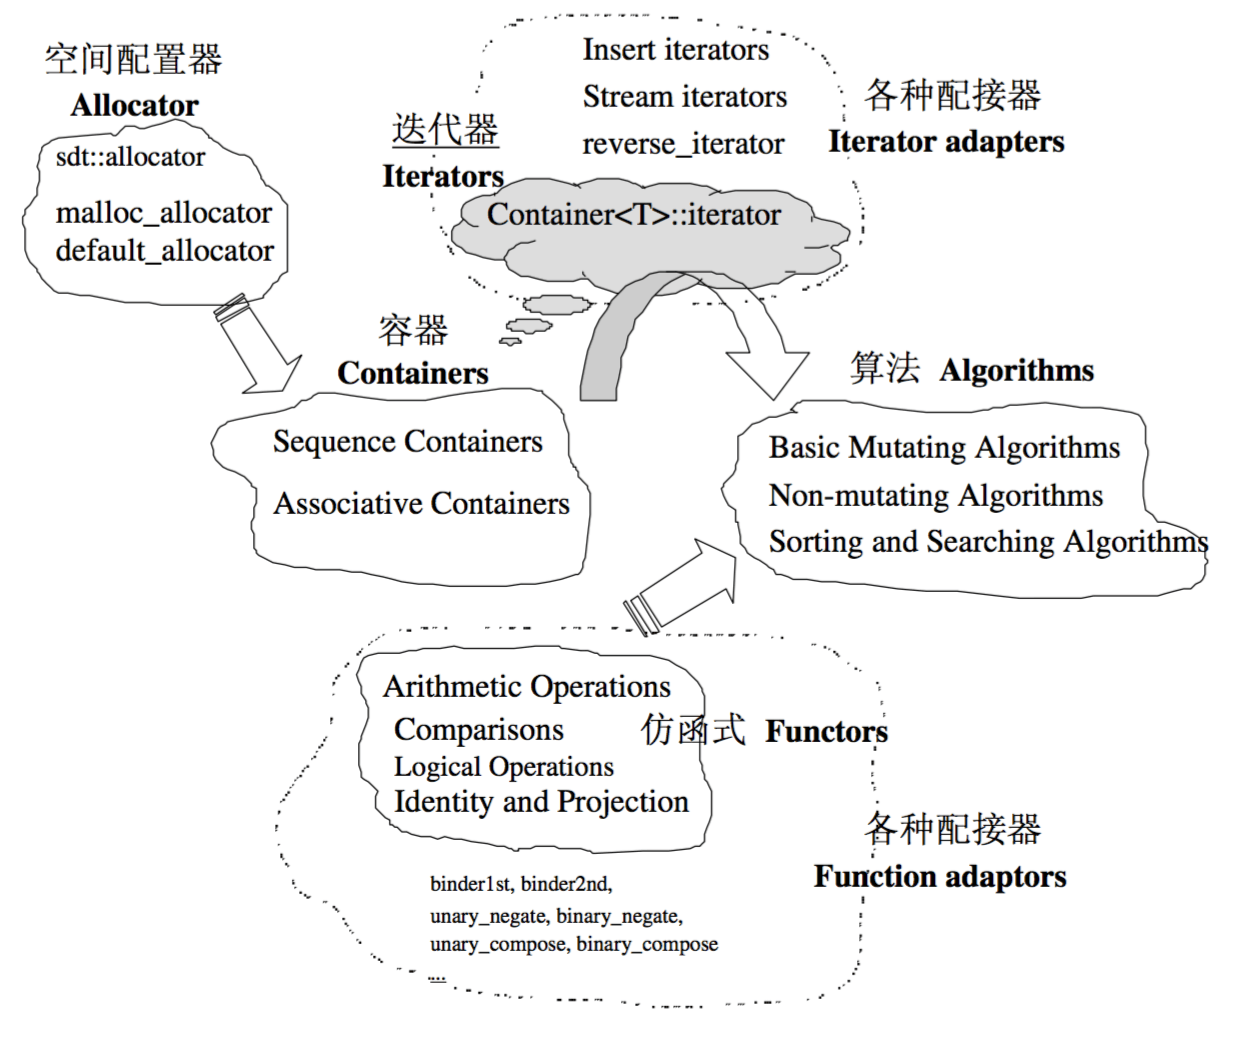
\includegraphics[width=0.75\textwidth]{CppSTL.png}
	\caption{六大组件的交互关系}
\end{figure}

\subsection {容器}

一个容器就是一些特定类型对象的集合。STL 中容器分为两大类,序列式容器和关联式容器。

序列式容器(sequential container)为程序员提供了控制元素存储和访问顺序的能力。这种顺序不依赖于元素的值,而是与元素加入容器时的位置相对应。

除了序列式容器容器外,标准库还定义了三个序列式容器适配器:stack、queue和priority_queue。适配器是标准库中的一个通用概念,容器、迭代器和函数都有适配器。本质上,一个适配器是一种机制,能使某种事物的行为看起来像另外一种事物一样。

和序列式容器对应的是关联容器(associative-container),关联容器中的元素是按关键字来保存和访问的。关联容器支持高效的关键字查找和访问,STL有两个主要的关联容器:map 和 set。

\subsubsection {顺序容器}

最简单的 STL 顺序容器就是 vector。Vector 只是一个拥有扩展功能的数组。

\begin{Code}
vector<int> v(10, 0);
int elements_count = v.size();
bool is_nonempty_ok = !v.empty();
\end{Code}

这里 V 包含了10 个 int 整数,初始化为0。Vector 最常使用的特性就是获取容器size,有两点要注意:首先,size() 函数返回的值是无符号的,这点有时会引起一些问题。其次,如果你想知道容器是否为空,把 size() 返回值和0比较不是一个好的做法。最好使用 empty() 函数,因为不是所有容器都能在常量时间内返回自己的大小,而且你绝不应该为了确定链表中至少包含一个节点元素就对一条双链表中的所有元素计数。

另一个 vector 中经常使用的函数是 push_back。Push_back 函数永远向 vector 尾部添加一个元素,容器长度加 1。当需要调整 vector 的大小时,使用 resize() 函数。如果在使用了 resize() 后又用了 push_back(),那新添加的元素就会位于新分配内存的后面,而不是被放入新分配的内存当中。

\begin{Code}
v.resize(15);
for(int i = 1; i < 5; i++) {
	v.push_back(i*2);
	//把元素写入下标值[15..20), not [10..15)
}
\end{Code}

向 vector 添加数据的最简单方式是使用 push_back()。但是,万一我们想在除了尾部以外的地方添加数据呢?Insert函数可以实现这个目的,往 vector 中插入一个元素:

\begin{Code}
vector<int> v(10,0);
v.insert(1, 42);    // Insert value 42 after the first
\end{Code}

从第二个(下标为1的元素)往后的所有元素都要右移一位,从而空出一个位置给新插入的元素。如果你打算添加很多元素,那多次右移并不可取——明智的做法是单次调用 insert(),指明插入数据的空间范围。

\begin{Code}
vector<int> v1(3,0);
vector<int> v2{1,2,3};
v1.insert(v1.begin(), v2.begin(), v2.end());
\end{Code}

还应该记住另一个非常重要的事情:当 vector 作为参数传给某个函数时,实际上是复制了这个 vector(也就是值传递)。在不需要这么做的时候创建新的 vector 可能会消耗大量时间和内存。实际上,很难找到一个任务需要在传递 vector 为参数时对其进行复制。所以,最好使用引用传递:

\begin{Code}
void some_function(const vector<int>& v) { 
	// Read only!
}
void some_function(vector<int>& v) { 
	// Can be Modified!
}
\end{Code}
此外,要知道我们可以创建任何类型的 vector,通过 vector 创建二维数组,最简单的方式就是创建一个存储 vector 元素的 vector。
\begin{Code}
int N=5, M=10;
vector< vector<int> > Matrix(N, vector<int>(M, -1));
\end{Code}
我们创建了一个 N * M 的矩阵,并用 -1 填充所有位置上的值。

erase()函数从指定容器删除指定位置的元素或某段范围内的元素,如果是删除指定位置的元素时,返回值是一个迭代器,指向删除元素下一个元素;如果是删除某范围内的元素时:返回值也表示一个迭代器,指向最后一个删除元素的下一个元素。

删除 vector 中指定的某个元素值(删除一个元素后导致后面所有的元素会向前移动一个位置):
\begin{Code}
vector<int> array = {1,2,6,6,7,8};
for (vector<int>::iterator itor = array.begin(); itor != array.end(); itor++)
{
	if (*itor == 6) {
		array.erase(itor);
		itor--;
	}
}
// 1,2,7,8
\end{Code}
其他的一些函数:
\begin{enumerate}
	\item   clear():清空 vector,使其包含 0 个元素,成为空容器。
	\item   capacity():返容器占用的内存空间,注意和v.size()的区别(空间的分配和size的关系);
	\item   pop_back():删除尾部的数据,size -= 1;
	\item   c.at(index):传回索引为index的数据,如果index越界,抛出out_of_range异常。
	\item   c.front():返回第一个数据。
	\item   c.back():传回最后一个数据,不检查这个数据是否存在。
\end{enumerate}

很多时候大量删除数据,或者通过使用reserver(),结果vector占有的空间远远大于实际的需要,这时候需要压缩vector到它的实际大小。在 C++11 中已经提供了shrink_to_fit()函数实现vector的压缩。
\begin{Code}
std::vector<int> v(1000,1);              // v.capacity()=1000
v.erase(v.begin(), v.begin()+v.size()/2);// v.capacity()=1000
v.shrink_to_fit();                       // v.capacity()=500
\end{Code}
(空间增长策略:按照容器现在容量的一倍进行增长。vector容器分配的是一块连续的内存空间,每次容器的增长,并不是在原有连续的内存空间后再进行简单的叠加,而是重新申请一块更大的新内存,并把现有容器中的元素逐个复制过去,然后销毁旧的内存。这时原有指向旧内存空间的迭代器已经失效,所以当操作容器时,迭代器要及时更新。)

\subsubsection {关联容器}

关联容器用来支持高效的关键字查找和访问,其中的元素是按照关键字来保存和访问的。与之相对,顺序容器中的元素是按它们在容器中的位置来顺序保存和访问的。两个主要的关联容器类型是 map 和 set:

 map中的元素是一些关键字-值对(key-value)对:关键字起到索引的作用,值则表示与索引相关联的数据。
 set中每个元素只包含一个关键字,set支持高效的关键字查询操作——检查一个给定关键字是否在 set 中。

标准库提供了8个关联容器,体现在三个不同的维度:

1. 或者是一个 map,或者是一个 set;

2. 允许关键字重复,或者不允许;

3. 按照顺序保存元素,或者无序保存。

具体情况如下表:

\begin{enumerate}
\item 定义关联容器

定义 map 必须指明关键字类型和值类型,而定义一个set时,只需要指明关键字类型。
\begin{Code}
map <string, size_t> word_count; // 空容器
set <string> exclude = {"the", "but", "and"}; // 列表初始化
map <string, string> authors = {{"Joyce", "James"},
	{"Austen", "Jane"}};
\end{Code}
对于有序容器,关键字类型必须定义元素比较的方法。默认情况下,标准库使用关键字类型的 < 运算符来比较两个关键字。

无序容器使用关键字类型的 == 运算符来比较元素,它们还使用一个hash<key_type>类型的对象来生成每个元素的哈希值。标准库为内置类型定义了 hash 模板,还为一些标准库类型,如 string 定义了hash。但是我们不能直接定义关键字类型为自定义类类型的无序容器。因为不能直接使用哈希模板,必须提供我们自己的 hash 模板版本。

\subitem pair类型

标准库类型 pair 是用来生成特定类型的模板,创建一个 pair 时必须提供两个类型名,pair的数据成员将具有对应的类型。
\begin{Code}
pair<string, string> anon{"James", "Joyce"};
pair<string, vector<int>> line;
\end{Code}
与其他标准库类型不同,pair的数据成员是 public 的,两个成员分别命名为 first 和 second,使用普通的成员访问符来访问它们。
\begin{Code}
cout << anon.first << anon.second;
\end{Code}

\item 关联容器操作

关联容器的类型有如下三个:
\begin{table}[hbp]
	\begin{tabular}{|c|l|}
		\hline
类型& 解释\\\hline
key_type &对应容器类型的关键字类型 \\ \hline
 mapped_type& map 关键字关联的类型 \\ \hline
 value_type& 对于 set,与 key_type 相同,对于map,为 pair<const key_type, mapped_type> \\ \hline
	\end{tabular}
\end{table}

解引用关联容器迭代器时,得到一个类型为容器的 value_type 的值的引用。对于map而言,value_type 是一个 pair 类型,其 first 成员保存 const 的关键字,second 成员保存值。

\begin{Code}
map<int, string> test{{1, "1"}};
auto iter = test.begin();
cout << iter->first << ", " << iter->second << endl;
// iter->first = 2;         // 关键字类型是 const 的
iter -> second = "2";
cout << iter->first << ", " << iter->second << endl;
\end{Code}

与不能改变 map 的关键字一样,一个 set 中的关键字也是 const 的,可以用一个 set 迭代器来读元素的值,但不能修改。

通常不对关联容器使用泛型算法,因为关键字是 const 这一特性意味着不能将关联容器传递给修改或者重排容器元素的算法(这类算法往往需要向元素写入值)。关联容器可用于只读取元素的算法。

\subitem \textbf{添加元素}

关联容器的 insert 成员向容器添加一个元素或一个元素的范围。insert 有两个版本,分别接受一对迭代器,或者是一个初始化器列表。注意,由于map 和 set 包含不重复的关键字,因此插入一个已经存在的元素对容器没有任何影响。
\begin{Code}
vector <int> ivec = {4,3,2,1,1,2,3,4};
set<int> set2;
set2.insert(ivec.cbegin(), ivec.cend());
// set2 = {1, 2, 3, 4} 有四个元素
\end{Code}
对 map 进行 insert 操作时,必须记住元素类型是 pair,一般在insert 参数列表中创建一个 pair:
\begin{Code}
map<string, int> word_count;
word_count.insert({"or", 1});
word_count.insert(make_pair("the", 1));
word_count.insert(pair<string, int>("and", 1));
word_count.insert(map<string, int>::value_type("text", 1));
\end{Code}
\subitem \textbf{检测 insert 的返回值}

insert 返回的值依赖于容器类型和参数,对于不包含重复关键字的容器,添加单一元素的 insert返回一个 pair,告诉我们插入操作是否成功。pair 的 first 成员是一个迭代器,指向具有给定关键字的元素,second 成员是一个 bool 值,指出元素是插入成功还是已经存在于容器中。
\begin{Code}
map<string, int> word_count;
word_count.insert({"or", 1});
auto ret = word_count.insert(make_pair("or", 1));
if(!ret.second){
	ret.first->second += 1;
}
// {"or", 2}
\end{Code}
我们要知道这里 ret 的类型为:
\begin{Code}
pair<map<string, int>::iterator, bool> 
\end{Code}
对允许重复关键字的容器,接受单个元素的 insert 操作返回一个指向新元素的迭代器,这里无需返回一个 bool值,因为 insert 操作总是向这类容器中加入一个新元素。

\subitem \textbf{删除元素}

关联容器定义了三个版本的 erase,与顺序容器一样,可以通过传递给 erase 一个迭代器删除一个元素或者一个迭代器对删除一个元素范围。这两个版本和顺序容器的操作类似,指定的元素被删除,返回 void。

此外,关联容器提供额外的 erase 操作,接受一个 key_type 参数,此版本删除所有匹配给定关键字的元素(如果存在的话),返回实际删除的元素的数量。对于保存不重复关键字的容器,erase返回值总是0或者1。

\subitem \textbf{map 的下标操作}

map 和 unordered_map 容器提供了下标运算符和一个对应的at函数。set类型不支持下标,因为set中没有与关键字相关联的值。也不能对 multimap 或 unordered_multimap 进行下标操作,因为这些容器中可能有多个值与一个关键字相关联。

如果关键字不在 map 中,会为它创建一个元素并插入到 map 中,关联值将进行值初始化。由于下标运算符可能插入一个新元素,我们只可以对非 const 的map使用下标操作。
\begin{Code}
map<string, int> word_count;
word_count["test"];
word_count["give"] = 1;
// word_count: {{give, 1},{test, 0}}
\end{Code}
上面最后一句执行的操作如下:

1. 在 word_count 中搜索关键字为 give 的元素,未找到;
2. 将一个新的关键字-值对插入到 word_count 中,关键字是一个 const string,保存 give,值进行初始化为0;
3. 提取出新插入的元素,并将值 1 赋予它。

对一个 map 进行下标操作时,会获得一个 mapped_type 对象。

\subitem \textbf{ 访问元素}

关联容器提供多种查找一个指定元素的方法,如果只关心一个特定元素是否已在容器中, find 是最佳选择。

|    操作     |   含义   |
|----------- |----------|
|  c.find(k) | 返回一个迭代器,指向第一个关键字为 k 的元素,若 k 不在容器中,则返回尾后迭代器 |
| c.count(k) | 返回关键字等于k的元素的数量,对于不允许重复关键字的容器,返回值永远是0或1    |
| c.lower_bound(k) | 返回一个迭代器,指向第一个关键字不小于 k 的元素| 
| c.upper_bound(k) | 返回一个迭代器,指向第一个关键字大于 k 的元素 |
| c.equal_range(k) | 返回一个迭代器 pair,表示关键字等于 k 的元素的范围。若 k 不存在,pair 的两个成员均等于 c.end() |

在一个不允许重复关键字的关联容器中查找一个元素是一件很简单的事情,元素要么在容器中,要么不在。但对于允许重复关键字的容器来说,过程更为复杂:容器中可能有很多元素具有给定的关键字。如果一个 multimap 或 multiset 中有多个元素具有给定关键字,则这些元素在容器中会相邻存储。
\begin{Code}
multimap<string, int> authors{{"Alain", 1}, {"Alain", 2}, {"Alain", 3}};
string search_item("Alain");
auto iter = authors.find(search_item);
auto entries = authors.count(search_item);
while(entries){
	cout << iter->second << endl;
	iter++;
	entries--;
}
\end{Code}
此外,可以用 lower_bound 和 upper_bound 来解决此类问题。 
\begin{Code}
for(auto beg = authors.lower_bound(search_item), end = authors.upper_bound(search_item);
beg != end; beg++){
	cout << beg->second << endl;
}
\end{Code}
\end{enumerate}

\subsection {迭代器}

迭代器提供对一个容器中的对象的访问方法,并且定义了容器中对象的范围。迭代器就如同一个指针。事实上,C++的指针也是一种迭代器。但是,迭代器不仅仅是指针,因此你不能认为他们一定具有地址值。例如,一个数组索引,也可以认为是一种迭代器。

迭代器有各种不同的创建方法。程序可能把迭代器作为一个变量创建。一个STL容器类可能为了使用一个特定类型的数据而创建一个迭代器。作为指针,必须能够使用操作符类获取数据。还可以使用其他数学操作符如++操作符用来递增迭代器,以访问容器中的下一个对象。如果迭代器到达了容器中的最后一个元素的后面,则迭代器变成past-the-end值。使用一个past-the-end值得指针来访问对象是非法的,就好像使用NULL或为初始化的指针一样。

对于STL数据结构和算法,可以使用五种迭代器。下面简要说明了这五种类型:

 Input iterators 提供对数据的只读访问
 
 Output iterators 提供对数据的只写访问
 
 Forward iterators 提供读写操作,并能向前推进迭代器
 
 Bidirectional iterators提供读写操作,并能向前和向后操作
 
 Random access iterators提供读写操作,并能在数据中随机移动


\subsection {算法}

STL通过函数模板提供了很多作用于容器的通用算法,例如查找、插入、删除、排序等,这些算法均需要引入头文件<algorithm>。

所有的 STL 算法都作用在由迭代器 [first, last) 所标示出来的区间上,可以分为两大类:

 质变算法(mutating algorithms):运算过程中会更改区间内迭代器所指的元素内容,如分割(partition)、删除(remove)等算法
 非质变算法(nonmutating algorithms):运算过程中不会更改区间内迭代器所指的元素内容,如匹配(search),计数(count)等算法

所有泛型算法的前两个参数都是一对迭代器,通常称为first和last,用以标示算法的操作区间。注意,将无效的迭代器传给某个算法,虽然是一种错误,但不保证能够在编译期间被捕捉出来。


\subsection {高效、安全使用 STL}

都是STL,可能写出来的效率相差几倍,所以要掌握写出高效 STL 代码的技巧。

\subsubsection {建立指针的容器}

当对象很大时,建立指针的容器而不是对象的容器,主要基于下面两个原因:

1. STL基于拷贝的方式的来工作,任何需要放入STL中的元素,都会被复制;这也好理解,STL工作的容器是在堆内开辟的一块新空间,而我们自己的变量一般存放在函数栈或另一块堆空间中。如果复制的对象很大,由复制带来的性能代价也不小;对于大对象的操作,使用指针来代替对象能消除这方面的代价;

2. 只涉及到指针拷贝操作,没有额外类的构造函数和赋值构造函数的调用。

下面例子:
\begin{Code}
	vector <BigObj> vt1;
	vt1.push_back(myBigObj);
	vector <BigObj* > vt2;
	vt2.push_back(new BigObj());
\end{Code}


不过要注意:

1. 容器销毁前需要自行销毁指针所指向的对象;否则就造成了内存泄漏;
2. 使用排序等算法时,需要构造基于对象的比较函数,如果使用默认的比较函数,其结果是基于指针大小的比较,而不是对象的比较;

\subsubsection {用区间成员函数}

尽量用区间成员函数代替单元素操作,使用区间成员函数有以下好处:

1. 更少的函数调用
2. 更少的元素移动
3. 更少的内存分配

例:将v2后半部的元素赋值给v1:

\begin{Code}
for (vector<Widget>::const_iterator ci = v2.begin() + v2.size() / 2;
ci != v2.end();
++ci)
v1.push_back(*ci);
// 使用区间成员函数assign()
v1.assign(v2.begin() + v2.size() / 2, v2.end());
\end{Code}

\subsubsection {避免 vector 频繁内存分配}

新增元素空间不够时,vector会进行如下操作:

1. 分配当前空间的两倍空间;

2. 将当前元素拷贝到新的空间中;

3. 释放之前的空间;

4. 将新值放入新空间指定位置;

如果预先知道空间的大小,预先分配空间(使用 reserve,或者定义 vector 时指明大小)避免了重新分配空间和复制的代价;注:reserve()只是修改了容量,并非大小,向vector中增加元素还是需要通过push_back加入;

\subsubsection {关联容器还是有序 vector}

对一些阶段性的操作:做一系列插入、完成之后,后续操作都是查询。使用vector有以下优势:

1. 因为可以对vector排序,关联容器带来的有序优势丧失;
2. 使用二分法查找的前提下,查询算法对连续的内存空间的访问要快于离散的空间;

\subsubsection {仿函数还是函数指针}

在仿函数(functor, 函数对象)的方式中,内联有效,而作为函数指针时,一般编译器都不会对函数指针指向的函数进行内联;即使指定了inline;

\begin{Code}
inline bool doubleGreater(double d1, double d2)
{
	return d1 > d2;
}
vector<double> v;
sort(v.begin(), v.end(), doubleGreater);
\end{Code}

这个调用不是真的把doubleGreater传给sort,它传了一个doubleGreater的指针。更好的方式是使用仿函数:

\begin{Code}
struct myclass {
	inline bool operator() (int i, int j) {
		return (i<j);
	}
} myobject;

sort(v.begin(), v.end(), myobject);
\end{Code}

\subsubsection {其它小条款}

1. 用empty()
 代替size()来检查是否为空。对于list,size()会遍历每一个元素来确定大小,时间复杂度 o(n),线性时间;而empty总是保证常数时间;
 
2. 尽量用成员函数代替同名的算法。基于效率考虑,成员函数知道自己这个容器和其他容器有哪些特有属性,能够利用到这些特性;而通用算法不可以;此外对于关联容器,成员函数find基于等价搜索,而通用算法find基于相等来搜索;可能导致结果不一样;

\subsection{参考}  

《STL 源码剖析》  

[标准模板库(STL)使用入门(上)](http://blog.jobbole.com/87586/)
  
[标准模板库(STL)使用入门(下)](http://blog.jobbole.com/88310/) 

[防止缓冲区溢出](http://www.ibm.com/developerworks/cn/security/buffer-defend/index.html)

[高效使用 STL](https://segmentfault.com/a/1190000002932246)  

[cplusplus:vector::reserve](http://www.cplusplus.com/reference/vector/vector/reserve/)
  
[C++ STL轻松导学](http://morningspace.51.net/resource/stlintro/stlintro.html)  

《C++ Primer》 11章:关联容器  

\section{C++编译和编译器}

\subsection{C++ 编译器工作原理}

简单地说,一个编译器就是一个程序,它可以阅读以某一种语言(源语言)编写的程序,并把该程序翻译成一个等价的、用另一种语言(目标语言)编写的程序。

C/C++编译系统将一个程序转化为可执行程序的过程包含:

\begin{itemize}
\item 预处理(preprocessing):根据已放置的文件中的预处理指令来修改源文件的内容。
\item 编译(compilation):通过词法分析和语法分析,在确认所有指令都是符合语法规则之后,将其翻译成等价的中间代码表示或汇编代码。
\item 汇编(assembly):把汇编语言代码翻译成目标机器指令的过程。
\item 链接(linking):找到所有用到的函数所在的目标文件,并把它们链接在一起合成为可执行文件(executable file)。
\end{itemize}


\subsubsection{预处理} 

预处理器是在程序源文件被编译之前根据预处理指令对程序源文件进行处理的程序。预处理器指令以\# 号开头标识,末尾不包含分号。预处理命令不是C/C++语言本身的组成部分,不能直接对它们进行编译和链接。C/C++语言的一个重要功能是可以使用预处理指令和具有预处理的功能。C/C++提供的预处理功能主要有文件包含、宏替换、条件编译等。

\begin{enumerate}
\item 文件包含

预处理指令 \# include 用于包含头文件,有两种形式:\# include <xxx.h>,\# include "xxx.h"。

尖括号形式表示被包含的文件在系统目录中。如果被包含的文件不一定在系统目录中,应该用双引号形式。在双引号形式中可以指出文件路径和文件名。如果在双引号中没有给出绝对路径,则默认为用户当前目录中的文件,此时系统首先在用户当前目录中寻找要包含的文件,若找不到再在系统目录中查找。

对于用户自己编写的头文件,宜用双引号形式。对于系统提供的头文件,既可以用尖括号形式,也可以用双引号形式,都能找到被包含的文件,但显然用尖括号形式更直截了当,效率更高。

\item 宏替换

\textbf{宏定义}:一般用一个短的名字代表一个长的代码序列。宏定义包括无参数宏定义和带参数宏定义两类。宏名和宏参数所代表的代码序列可以是任何意义的内容,如类型、常量、变量、操作符、表达式、语句、函数、代码块等。

宏定义在源文件中必须单独另起一行,换行符是宏定义的结束标志,因此宏定义以换行结束,不需要分号等符号作分隔符。如果一个宏定义中代码序列太长,一行不够时,可采用续行的方法。续行是在键入回车符之前先键入符号\\,注意回车要紧接在符号\\之后,中间不能插入其它符号,当然代码序列最后一行结束时不能有\\。

预处理器在处理宏定义时,会对宏进行展开(即\textbf{宏替换})。宏替换首先将源文件中在宏定义随后所有出现的宏名均用其所代表的代码序列替换之,如果是带参数宏则接着将代码序列中的宏形参名替换为宏实参名。宏替换只作代码字符序列的替换工作,不作任何语法的检查,也不作任何的中间计算,一切其它操作都要在替换完后才能进行。如果宏定义不当,错误要到预处理之后的编译阶段才能发现。

\item 条件编译

一般情况下,在进行编译时对源程序中的每一行都要编译,但是有时希望程序中某一部分内容只在满足一定条件时才进行编译,如果不满足这个条件,就不编译这部分内容,这就是\textbf{条件编译}。

条件编译主要是进行编译时进行有选择的挑选,注释掉一些指定的代码,以达到多个版本控制、防止对文件重复包含的功能。if, \# ifndef, \# ifdef, \# else, \# elif, \# endif是比较常见条件编译预处理指令,可根据表达式的值或某个特定宏是否被定义来确定编译条件。

此外,还有 \# pragma 指令,它的作用是设定编译器的状态或指示编译器完成一些特定的动作。
\end{enumerate}
\subsubsection{编译} 

编译过程的第一个步骤称为词法分析(lexical analysis)或扫描(scanning),词法分析器读入组成源程序的字符流,并且将它们组织成有意义的词素的序列,对于每个词素,词法分析器产生一个词法单元(token),传给下一个步骤:语法分析。

语法分析(syntax analysis)或解析(parsing)是编译的第二个步骤,使用词法单元来创建树形的中间表示,该中间表示给出了词法分析产生的词法单元流的语法结构。一个常用的表示方法是语法树(syntax tree),树中每个内部结点表示一个运算,而该结点的子结点表示该运算的分量。

接下来是语义分析(semantic analyzer),使用语法树和符号表中的信息来检测源程序是否和语言定义的语义一致。

在源程序的语法分析和语义分析之后,生成一个明确的低级的或者类机器语言的中间表示。接下来一般会有一个机器无关的代码优化步骤,试图改进中间代码,以便生成更好的目标代码。

\subsubsection{汇编} 

对于被翻译系统处理的每一个C/C++语言源程序,都将最终经过这一处理而得到相应的目标文件。目标文件中所存放的也就是与源程序等效的目标机器语言代码。目标文件由段组成,通常一个目标文件中至少有两个段:代码段和数据段。

\begin{itemize}
\item 代码段:该段中所包含的主要是程序的指令。该段一般是可读和可执行的,但一般却不可写。
\item 数据段:主要存放程序中要用到的各种全局变量或静态的数据。一般数据段都是可读,可写,可执行的。
\end{itemize}

\subsubsection{链接} 

链接程序的主要工作就是将有关的目标文件彼此相连接,也即将在一个文件中引用的符号同该符号在另外一个文件中的定义连接起来,使得所有的这些目标文件成为一个能够按操作系统装入执行的统一整体。主要有静态链接和动态链接两种方式:

\begin{itemize}
\item 静态链接:在链接阶段,会将汇编生成的目标文件.o与引用到的库一起链接打包到可执行文件中,程序运行的时候不再需要静态库文件。
\item 动态链接:把调用的函数所在文件模块(DLL)和调用函数在文件中的位置等信息链接进目标程序,程序运行的时候再从DLL中寻找相应函数代码,因此需要相应DLL文件的支持。  
\end{itemize}

这里的库是写好的现有的,成熟的,可以复用的代码。现实中每个程序都要依赖很多基础的底层库,不可能每个人的代码都从零开始,因此库的存在意义非同寻常。本质上来说库是一种可执行代码的二进制形式,可以被操作系统载入内存执行。库有两种:静态库(.a、.lib)和动态库(.so、.dll),所谓静态、动态是指链接方式的不同。

静态链接库与动态链接库都是\textbf{共享代码}的方式。如果采用静态链接库,程序在运行时与函数库再无瓜葛,移植方便。但是会浪费空间和资源,因为所有相关的目标文件与牵涉到的函数库被链接合成一个可执行文件。此外,静态库对程序的更新、部署和发布也会带来麻烦。如果静态库更新了,所有使用它的应用程序都需要重新编译、发布给用户。

动态库在程序编译时并不会被连接到目标代码中,而是在程序运行是才被载入。不同的应用程序如果调用相同的库,那么在内存里只需要有一份该共享库的实例,规避了空间浪费问题。动态库在程序运行是才被载入,也解决了静态库对程序的更新、部署和发布页会带来麻烦。用户只需要更新动态库即可,增量更新。

此外,还要注意静态链接库中不能再包含其他的动态链接库或者静态库,而在动态链接库中还可以再包含其他的动态或静态链接库。

\subsubsection{简单的例子} 

下面是一个保存在文件 helloworld.cpp 中一个简单的 C++ 程序的代码:
\begin{Code}
    /* helloworld.cpp */
    #include <iostream>
    int main(int argc,char *argv[])
    {
        std::cout << "hello, world" << std::endl;
        return 0;
    }
\end{Code}

用下面命令编译:
\begin{Code}
    $ g++ helloworld.cpp
\end{Code}

编译器 g++ 通过检查命令行中指定的文件的后缀名可识别其为 C++ 源代码文件。编译器默认的动作:编译源代码文件生成对象文件(object file),链接对象文件和 libstd c++ 库中的函数得到可执行程序,然后删除对象文件。由于命令行中未指定可执行程序的文件名,编译器采用默认的 a.out。

\begin{enumerate}

\item 预处理

\textbf{选项 -E} 

使 g++ 将源代码用编译预处理器处理后不再执行其他动作。下面的命令预处理源码文件 helloworld.cpp,并将结果保存在 .ii 文件中:

\begin{Code}
    ➜  ~  g++ -E helloworld.cpp -o helloworld.ii
    ➜  ~  ls | grep helloworld
    helloworld.cpp
    helloworld.ii
    ➜  ~  wc -l helloworld.ii
       38126 helloworld.ii
\end{Code}
helloworld.cpp 的源代码,仅仅有六行,而且该程序除了显示一行文字外什么都不做,但是,预处理后的版本将超过3万行。这主要是因为头文件 iostream 被包含进来,而且它又包含了其他的头文件,除此之外,还有若干个处理输入和输出的类的定义。

\item  编译

\textbf{选项 -S} 

指示编译器将程序编译成汇编代码,输出汇编语言代码而后结束。下面的命令将由 C++ 源码文件生成汇编语言文件 helloworld.s,生成的汇编语言依赖于编译器的目标平台。

\begin{Code}
    g++ -S helloworld.cpp
\end{Code}

\item  汇编

\textbf{选项 -c}

 用来告诉编译器将汇编代码(.s文件,或者直接对源代码)转换为目标文件,但不要执行链接。输出结果为对象文件,文件默认名与源码文件名相同,只是将其后缀变为 .o。

\begin{Code}
    ➜  ~  g++ -c helloworld.s
    ➜  ~  ls |grep helloworld.o
    helloworld.o
\end{Code}

\item  链接

加载相应的库,执行链接操作,将对象文件(.o,也可以直接将原文件)转化成可执行程序。

\begin{Code}
    ➜  ~  g++ helloworld.o -o helloworld.o
    ➜  ~  ./helloworld.o
    hello, world 
\end{Code}
\end{enumerate}

\subsubsection{参考} 
 
[详解C/C++预处理器](http://blog.csdn.net/huang_xw/article/details/7648117)  

[Compiling Cpp](http://wiki.ubuntu.org.cn/Compiling_Cpp)
  
[C++静态库与动态库](http://www.cnblogs.com/skynet/p/3372855.html)  

[高级语言的编译:链接及装载过程介绍](http://tech.meituan.com/linker.html)  
  
[编译原理](http://www.cnblogs.com/pipicfan/archive/2012/07/10/2583910.html) 
 


